\documentclass[a4paper,11pt]{article}
\usepackage[T1]{fontenc}
\usepackage[utf8]{inputenc}
\usepackage{lmodern}
\usepackage{graphicx}
\usepackage[top=2cm, bottom=2cm, left=2cm, right=2cm]{geometry}
\usepackage{subcaption}
\usepackage{hyperref}

\title{INFO-F-404~: Real-Time Operating Systems\\Project 2~: Bitonic}
\author{Rémy Detobel, Stanislas Gueniffey and Denis Hoornaert}

\begin{document}

\maketitle

\section{Implementation choices}

  There are two main types of processes~: one \textit{master node} and multiple \textit{compute nodes}. Each node has its own purpose and interacts with the other processes using \textit{MPI}. Inside the code, the \texttt{main} function assigns a type to the current process, by calling the \texttt{masterNode} function if the process's rank is 0, and the \texttt{computeNode} function otherwise. We have implemented the bonus part with the same code basis as the main part, please refer to section \ref{usage} to learn about the its usage.

\subsection{Master}\label{master-node}
  \noindent The objective of the \textit{master node} is to synchronize and deal \textit{merge tasks} to the \textit{compute nodes}. It does so by executing one or more successive \texttt{masterMerge} calls, which consist of sending two values to each \textit{compute node}, and receiving back two values. Here is an example of an execution of \texttt{masterMerge}~:
  \begin{enumerate}
  \item $size$ is inferred from the sequence size and the goal (more on that later)
  \item for each \textit{compute node}, identified by $i = rank-1$:
  \begin{enumerate}
  	\item send values $(v_k, v_l)$ to $i$, where $$k = \left \lfloor{\frac{i}{size/2}} \right \rfloor \cdot size + (i\;mod\;size)\;, \qquad l = k+\frac{size}{2}$$
    \item receive values from $i$, and place them at indexes $(2*i, 2*i+1)$ of the sequence
  \end{enumerate}
  \end{enumerate}
  More precisely, if the goal is to sort an arbitrary list, N calls will be made : the first N-1 will result in the sequence being bitonic, and the last will ensure the sequence is sorted. In that case the value $size$ will be initialized at $2$ and then doubled for each call, until reaching the size of the sequence. If instead the goal is to sort a provided bitonic sequence, only one call will be required, with $size$ initialized as the sequence size.\\
  
  \noindent The intuition of the \texttt{masterMerge} function is that it executes the first and last steps of the \texttt{Merge 2k} algorithm seen in the course, all other steps being executed by the \textit{compute} nodes. The way $k$ and $l$ are computed allows us to parallelize multiple independent executions of the \texttt{Merge 2k} algorithm on increasingly large independent subsets of the sequence, until we can run a single instance over the whole sequence. The  $\left \lfloor{\frac{i}{size/2}} \right \rfloor \cdot size$ factor of $k$ is what separates these subsets, and always equals $0$ in the last call.
  
\subsection{Compute}
  \noindent The purpose of the \textit{compute nodes} is to compare pairs of values and to determine to which other \textit{compute node} they have to send the outcome of the comparison to. The mechanism is defined in the \texttt{computeMerge} function and works as follows~:
  \begin{enumerate}
  \item \textit{compute node} $i = rank-1$ receives values $(v_0, v_1)$ from the master node
  \item the value $depth$ is inferred from the sequence size and the selected outcome
  \item values are reordered according to order $O$, which can be assumed to be non-decreasing order for now
  \item if depth equals $0$, send both ordered values to the \textit{master node}
  \item the rank of a \textit{paired process} $i'$ is determined using the formula $$i' = i \oplus 2^{depth}$$
  \item the value to send and replace with value from $i'$ is $v_l$ where $l$ is the $(depth-1)^{th}$ least significant bit in the binary unsigned integer representation of $i$. 
  \item the selected value is sent and replaced by the value received from $i'$
  \item $depth$ is decreased and the process is repeated from step $3$
  \end{enumerate}
  
  \noindent This \texttt{computeMerge} function is called exactly once for each \texttt{computeMerge} call. It is easy to verify that the number of calls does not depend on the values to sort, only on the size of the sequence (which is known by all processes since it only depends on the total number of processes). In each of these successive calls, the initial value of $depth$ is set to match $log_2(size)-1$. That value then represents the comparisons left to perform, and is decreased after each loop.\\
  
  \noindent The intuition of \texttt{computeMerge} is that is executes a generalized version of the \texttt{Merge 2k} algorithm. After each comparison, processes split into two independent groups (of size $2^{depth}$), and the distance between compared values is divided by two. By that logic, the \textit{paired} process is simply the process that will have the same relative position in the other group after the split, and which needs the result of the comparison. When a group splits, in order to avoid unnecessary interactions, the lower half of the processes hangs on to their (consecutive) $v_0$ values whilst the rest keep their (consecutive) $v_1$ values, leaving two (consecutive) sub-sequences of values to exchange in total. Finally, the order $O$ of the comparison is the desired order of the list, but it is inverted in alternate groups during the \texttt{computeMerge} calls used to turn a sequence bitonic.\\
  
  \noindent Figure \ref{fig:bitonic_wiki} shows the complete sequence of comparisons involved in the bitonic sort for an arbitrary sequence of size 16. Arrows represent compare-swap instructions, and point towards the resulting $v_1$. It features four boxes corresponding to four calls to \texttt{masterMerge} and \texttt{computeMerge}. Withing each box, stacks of red sub-boxes are independent groups or processes. The background indicades if the order of the comparison is normal (blue) or reversed (green).

\begin{figure}[!h]
  \centering
  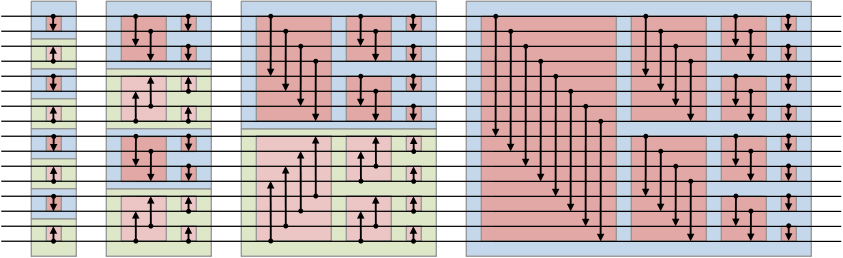
\includegraphics[width=\textwidth]{img/bitonic.png}
  \caption{Network representation of the complete bitonic sort (16 inputs)}
  \label{fig:bitonic_wiki}
\end{figure}


\section{Project usage and configuration}\label{usage}

  As mentioned in the assignment statements, the source code can either be used with a \textit{bitonic} list as input or with an unsorted list.\\
  However, unlike what has been specified in the assignment statement, there is only one source code as the project implement a general way to resolve both the mandatory and the bonus part (i.e. providing two separate files would have been equivalent to a copy-paste). In order to get the two executables, the user is invited to use the provided makefile, two executable will be named respectively \verb|bitonic| for the mandatory part of the project and \verb|bitonicbonus| for the bonus part of the project.

\section{Inter-processes communications}

  The implemented inter-processes communication protocol (\ref{fig:sato_comm}) differs a bit from the one suggested in the reference (\ref{fig:impl_comm}). In fact, in order to ease the implementation of the \textit{parallel bitonic sorting algorithm} and to preserve the \texttt{merge} functions used for sorting bitonic sequences intact, it has been decided that after each merge the \textit{compute nodes} have to send their results to the master node instead of dealing themselves with the communication. Consequently, parallelism is not exploited as far as possible and this has an impact on the expected performances.
  \begin{figure}[h!]
    \centering
    \begin{subfigure}[b]{0.4\textwidth}
        \centering
        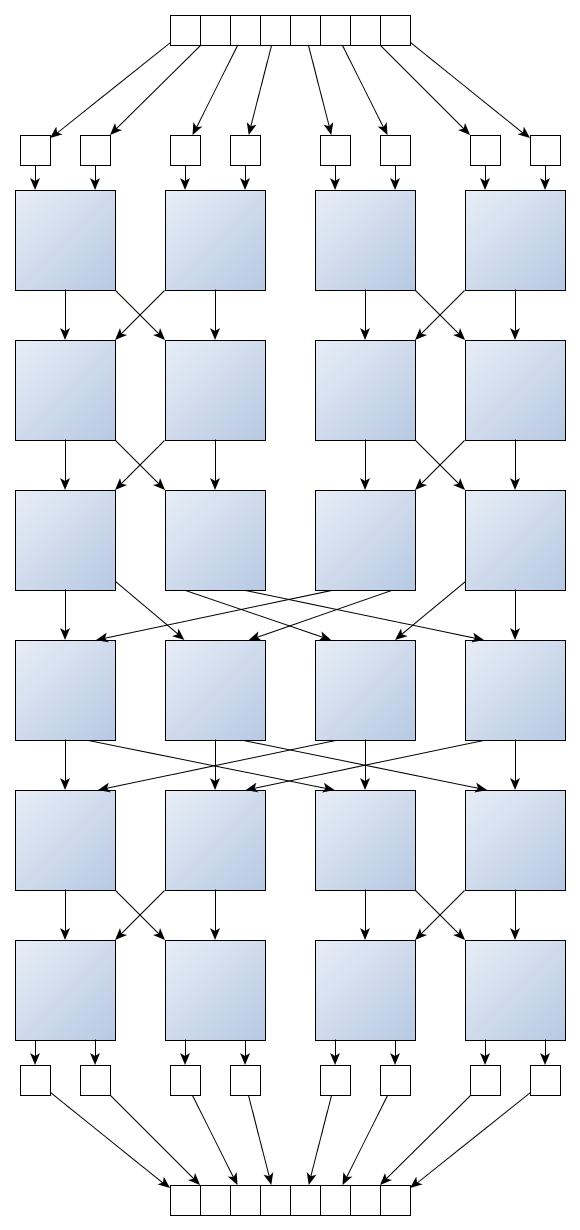
\includegraphics[scale=0.15]{img/bitonic_sort_8_sota.png}
        \caption{State of the art commnucations}
        \label{fig:sato_comm}
    \end{subfigure}
    ~
    \begin{subfigure}[b]{0.4\textwidth}
        \centering
        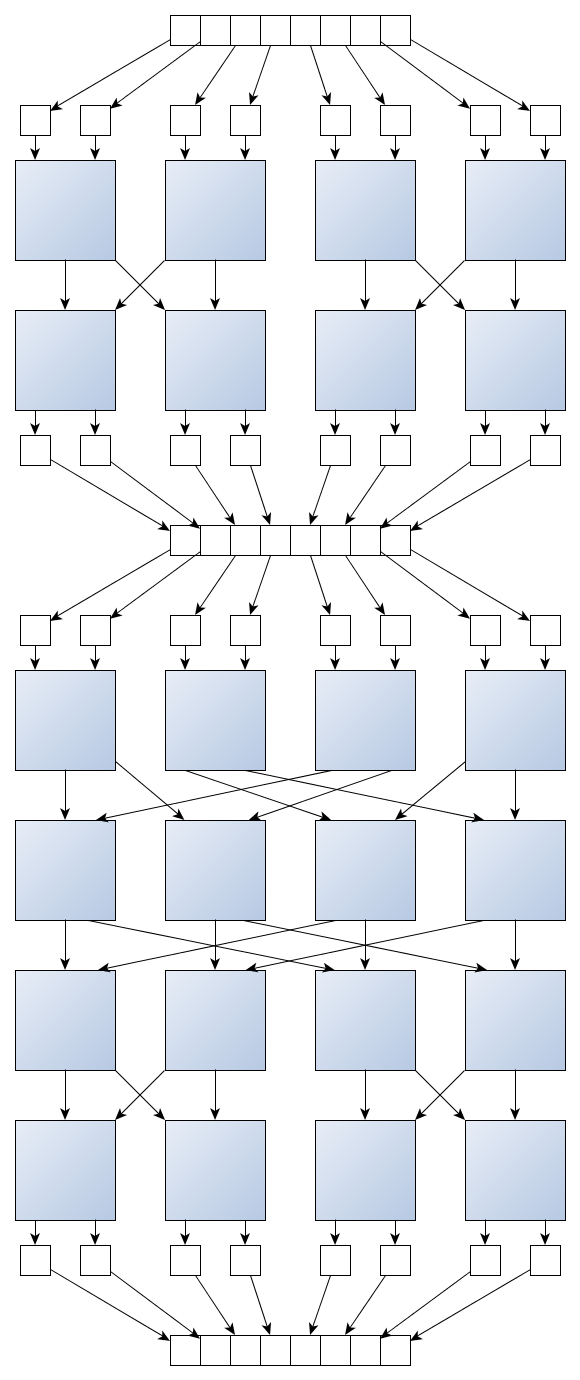
\includegraphics[scale=0.15]{img/bitonic_sort_8.png}
        \caption{Project communications}
        \label{fig:impl_comm}
    \end{subfigure}
    \caption{}
    \label{}
  \end{figure}

\section{Limitations and performances}

  The biggest limitation of the project is due to the inter-node communication protocol that has been implemented. For reminder, the \textit{master node} oversees the important steps of the communication scheme (See section \ref{master-node} for further information).
  Even though introducing such a protocol has eased the development of the project, useless communications have also been introduced resulting in an non-optimal (but more than correct) use of \textit{MPI}.
  This flaw could be addressed by implementing a formula that would deterministically choose the correct destination ($=$ \textit{compute node}). Consequently, the \textit{master node} would be less solicited as it would not have to oversee the communications anymore (i.e. its job would only consists of sending the initial list and receiving the sorted list).\\
  
  \noindent Further more, provided that the above "optimisation" has been implemented, one could also consider using the master mode as a \textit{computation node}. There would be several benefits as the overall number of required communications would decrease and as the number of required processes would be reduced by 1. Notice that this "optimisation" would however breaks one of the rules of the assignment statement.

\section{Encountered difficulties}

  Regardless of the difficulties that directly involved \textit{MPI}, the main difficulties encountered during the realisation of the project have been the derecurssivication of the \textit{classic} \textit{bitonic sort} and the distribution of the comparisons modules into several processes. 

\end{document}
